\PassOptionsToPackage{enable-debug,check-declarations}{expl3}
\RequirePackage{pdfmanagement-testphase}
\DeclareDocumentMetadata {  }
\ExplSyntaxOn
\pdfmanagement_add:nnn{Catalog}{Lang}{(enUS)}
\ExplSyntaxOff

% xmp metadata for pdf
% Originally used \usepackage[a-2a]{pdfx}
% \usepackage{hyperxmp} replaced it
% \RequirePackage{pdfmanagement-testphase} replaced it

\documentclass[11pt,
  english,
  a4paper,
]{article}
\usepackage{sa4ss}
\usepackage{amsmath,amssymb,array}
\usepackage{booktabs}

% From tagged-template.latex
\usepackage{lmodern}
\usepackage{ifxetex,ifluatex}
\ifnum 0\ifxetex 1\fi\ifluatex 1\fi=0 % if pdftex
  \usepackage[T1]{fontenc}
  \usepackage[utf8]{inputenc}
  \usepackage{textcomp} % provide euro and other symbols
\else % if luatex or xetex
  \usepackage{unicode-math}
  \defaultfontfeatures{Scale=MatchLowercase}
  \defaultfontfeatures[\rmfamily]{Ligatures=TeX,Scale=1}
\fi

% Use upquote if available, for straight quotes in verbatim environments
\IfFileExists{upquote.sty}{\usepackage{upquote}}{}
\IfFileExists{microtype.sty}{% use microtype if available
  \usepackage[]{microtype}
  \UseMicrotypeSet[protrusion]{basicmath} % disable protrusion for tt fonts
}{}
\makeatletter
\@ifundefined{KOMAClassName}{% if non-KOMA class
  \IfFileExists{parskip.sty}{%
    \usepackage{parskip}
  }{% else
    \setlength{\parindent}{0pt}
    \setlength{\parskip}{6pt plus 2pt minus 1pt}}
}{% if KOMA class
  \KOMAoptions{parskip=half}}
\makeatother
\usepackage{xcolor}
\IfFileExists{xurl.sty}{\usepackage{xurl}}{} % add URL line breaks if available
\hypersetup{
  pdftitle={DRAFT The status of Vermilion Rockfish (Sebastes miniatus) and Sunset Rockfish (Sebastes crocotulus) in U.S. waters off the coast of California south of Pt. Conception in 2021},
  pdflang={en},
  hidelinks,
  pdfcreator={LaTeX via pandoc}}
\urlstyle{same} % disable monospaced font for URLs
\usepackage{longtable}
% Correct order of tables after \paragraph or \subparagraph
\usepackage{etoolbox}
\makeatletter
\patchcmd\longtable{\par}{\if@noskipsec\mbox{}\fi\par}{}{}
\makeatother
% Allow footnotes in longtable head/foot
\IfFileExists{footnotehyper.sty}{\usepackage{footnotehyper}}{\usepackage{footnote}}
\makesavenoteenv{longtable}
\usepackage{graphicx}
\makeatletter
\def\maxwidth{\ifdim\Gin@nat@width>\linewidth\linewidth\else\Gin@nat@width\fi}
\def\maxheight{\ifdim\Gin@nat@height>\textheight\textheight\else\Gin@nat@height\fi}
\makeatother
% Scale images if necessary, so that they will not overflow the page
% margins by default, and it is still possible to overwrite the defaults
% using explicit options in \includegraphics[width, height, ...]{}
\setkeys{Gin}{width=\maxwidth,height=\maxheight,keepaspectratio}
% Set default figure placement to htbp
\makeatletter
\def\fps@figure{htbp}
\makeatother
\setlength{\emergencystretch}{3em} % prevent overfull lines
\providecommand{\tightlist}{%
  \setlength{\itemsep}{0pt}\setlength{\parskip}{0pt}}
\setcounter{secnumdepth}{5}
\usepackage{booktabs}
\usepackage{longtable}
\usepackage{array}
\usepackage{multirow}
\usepackage{wrapfig}
\usepackage{float}
\usepackage{colortbl}
\usepackage{pdflscape}
\usepackage{tabu}
\usepackage{threeparttable}
\usepackage[normalem]{ulem}
\usepackage{makecell}
\usepackage{placeins}
\ifxetex
  % Load polyglossia as late as possible: uses bidi with RTL langages (e.g. Hebrew, Arabic)
  \usepackage{polyglossia}
  \setmainlanguage[]{english}
\else
  \usepackage[shorthands=off,main=english]{babel}
\fi

%Define cslreferences environment, required by pandoc 2.8
%https://github.com/rstudio/rmarkdown/issues/1649


\providecommand{\tightlist}{%
  \setlength{\itemsep}{0pt}\setlength{\parskip}{0pt}}

\usepackage{booktabs}
\usepackage{longtable}
\usepackage{array}
\usepackage{multirow}
\usepackage{wrapfig}
\usepackage{float}
\usepackage{colortbl}
\usepackage{pdflscape}
\usepackage{tabu}
\usepackage{threeparttable}
\usepackage[normalem]{ulem}
\usepackage{makecell}
\usepackage{placeins}
\date{}
\newcommand{\trTitle}{DRAFT The status of Vermilion Rockfish (\emph{Sebastes miniatus}) and Sunset Rockfish (\emph{Sebastes crocotulus}) in U.S. waters off the coast of California south of Pt. Conception in 2021}
\newcommand{\trYear}{2021}
\newcommand{\trMonth}{August}
\newcommand{\trAuthsLong}{truetruetruetruetrue}
\newcommand{\trAuthsBack}{Dick, E.J., M.H. Monk, T.L. Rogers, J.C. Field, E.M. Saas}
\newcommand{\trCitation}{
\begin{hangparas}{1em}{1}
\trAuthsBack{}. \trYear{}. \trTitle{}. Pacific Fisheries Management Council, Portland, Oregon. \pageref{LastPage}{}\,p.
\end{hangparas}}

\AtBeginDocument{\tagstructbegin{tag=Document}}
\AtEndDocument{\tagstructend}
\pretocmd{\maketitle}{\tagstructbegin{tag=H1}\tagmcbegin{tag=H1}}{}{}
\apptocmd{\maketitle}{\tagmcend\tagstructend}{}{}

\begin{document}

%%%%% Frontmatter %%%%%

% Footnote symbols in front matter
\renewcommand*{\thefootnote}{\fnsymbol{footnote}}

\small
\thispagestyle{empty}
\pagenumbering{roman}
\noindent
\begin{center}
\title{DRAFT The status of Vermilion Rockfish (\emph{Sebastes miniatus}) and Sunset Rockfish (\emph{Sebastes crocotulus}) in U.S. waters off the coast of California south of Pt. Conception in 2021}
% \textnormal{\MakeTextUppercase{\trTitle{}}}
\vspace{1.5cm}
{\Large\textbf\newline{DRAFT The status of Vermilion Rockfish (\emph{Sebastes miniatus}) and Sunset Rockfish (\emph{Sebastes crocotulus}) in U.S. waters off the coast of California south of Pt. Conception in 2021}}
\vfill
by\\
E. J. Dick\textsuperscript{1}\\
Melissa H. Monk\textsuperscript{1}\\
Tanya L. Rogers\textsuperscript{1}\\
John C. Field\textsuperscript{1}\\
Emma M. Saas\textsuperscript{2}\vfill
\textsuperscript{1}Southwest Fisheries Science Center, U.S. Department of Commerce, National Oceanic and Atmospheric Administration, National Marine Fisheries Service, 110 McAllister Way, Santa Cruz, California 95060\\
\textsuperscript{2}Fisheries Collaborative Program, Insitute of Marine Sciences, University of California, Santa Cruz, 110 McAllister Way, Santa Cruz, California 95060\vfill
\trMonth{} \trYear{}
\end{center}
\clearpage

% Fourth page: Colophon
\thispagestyle{empty}
\vspace*{\fill}
\begin{center}
\copyright{} Pacific Fisheries Management Council, \trYear{}\\
\end{center}
\par
\bigskip
\noindent
Correct citation for this publication:
\bigskip
\par
\trCitation{}
\clearpage

% Add TOC to pdf bookmarks (clickable pdf)
\pdfbookmark[1]{\contentsname}{toc}

% Table of contents page, lists of figures and tables
\tableofcontents\clearpage
\label{TRlastRoman}
\clearpage

% Table of contents
\newpage
\thispagestyle{empty} % to remove page number

% Settings for the main document
\pagenumbering{arabic}  % Regular page numbers
\pagestyle{plain}  % No page number on first page of main document, use 'empty'
\renewcommand*{\thefootnote}{\arabic{footnote}}  % Back to numeric footnotes
\setcounter{footnote}{0}  % And start at 1
\renewcommand{\headrulewidth}{0.5pt}
\renewcommand{\footrulewidth}{0.5pt}
%\pagestyle{fancy}\fancyhead[c]{Draft: Do not cite or circulate}

\newcommand{\lt}{\ensuremath <}
\newcommand{\gt}{\ensuremath >}

\newcommand\CapeM{$40^\circ 10^\prime N$}
\newcommand\PtC{$34^\circ 27^\prime N$}
\newcommand\CAOR{$42^\circ 00^\prime N$}

\newpage

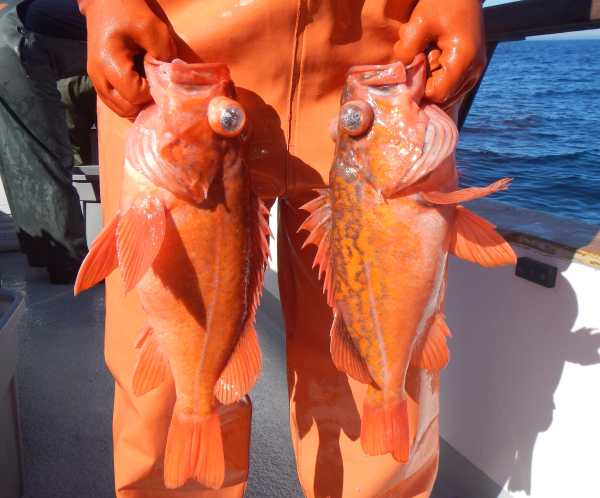
\includegraphics{cover_photo.png} Two fish of the vermilion/sunset cryptic species pair. Confirmation of species can only be determined via genetic analysis and species identification of these two fish caught in the Santa Barbara channel at approximately 250 ft depth is unknown. Photo courtesy of Sabrina Beyer (UCSC/NOAA).

\pagebreak
\pagenumbering{roman}
\setcounter{page}{1}

\renewcommand{\thetable}{\roman{table}}
\renewcommand{\thefigure}{\roman{figure}}

\setlength\parskip{0.5em plus 0.1em minus 0.2em}

\tagstructbegin{tag=H1}\tagmcbegin{tag=H1}

\hypertarget{executive-summary}{%
\section*{Executive Summary}\label{executive-summary}}
\addcontentsline{toc}{section}{Executive Summary}

\leavevmode\tagmcend\tagstructend

\tagstructbegin{tag=H2}\tagmcbegin{tag=H2}

\hypertarget{stock}{%
\subsection*{Stock}\label{stock}}
\addcontentsline{toc}{subsection}{Stock}

\leavevmode\tagmcend\tagstructend

This assessment reports the combined status of the vermilion rockfish (\emph{Sebastes miniatus}) and sunset rockfish (\emph{Sebastes crocotulus}), referred to as ``vermilion rockfish'' throughout, in U.S. waters off the coast of California south of Point Conception ($34^\circ 27^\prime N$) using data through 2020. Genetic evidence suggests overlapping distributions for the two species, with the majority of the sunset rockfish population occupying waters south of Point Conception. Alternative spatial structures for the vermilion rockfish assessment should be considered if additional data on stock structure and the distribution of the two species become available.

\tagstructbegin{tag=H2}\tagmcbegin{tag=H2}

\hypertarget{catches}{%
\subsection*{Catches}\label{catches}}
\addcontentsline{toc}{subsection}{Catches}

\leavevmode\tagmcend\tagstructend

Over the past decade, vermilion rockfish in the assessed area off the coast of California in have been primarily caught by the recreational fishery (Table \ref{tab:removalsES}). Annual total mortality of catch and discards of vermilion rockfish have ranged between 106-260 mt, with total mortality (catch + discards) in 2020 of 110 mt. Vermilion and sunset rockfishes landings from all sectors have historically been recorded as ``vermilion rockfish'' and sampling programs in California currently do not differentiate between the two species.

Recreational removals in California prior to 2004 were only estimated at large spatial scales (north and south of Point Conception) following the design of the Marine Recreational Fisheries Statistics Survey (MRFSS). Recent sampling (2004 -- present) by the California Recreational Fisheries Survey (CRFS) produces estimates of vermilion landings and discard at a finer spatial resolution. Total removals south of Point Conception increased steadily following World War II, peaking in the late 1970s and 1980s with annual removals exceeding 398 mt per year (Figure \ref{fig:catch}). Recent years have seen a steady increase in landings, with recreational fleets accounting for the majority of landings.

\FloatBarrier

\begin{figure}
\centering
\includegraphics[width=1\textwidth,height=1\textheight]{C:/Stock_Assessments/VRML_Assessment_2021/Model_files/SCA/Verm21SoCA_089_pre-STAR_base_with_SS_OPT/plots/catch2 landings stacked.png}
\caption{Catch histories by fleet used in the base model (Commercial hook-and-line = COM\_HKL, Commercial trawl = COM\_TWL, Commercial net = COM\_NET, Recreational party/charter retained = REC\_PC, Recreational private/rental retained = REC\_PR, Recreational party/charter dead discards = REC\_PC\_DIS, Recreational private/rental dead discards = REC\_PR\_DIS).\label{fig:catch}}
\end{figure}

\begin{table}[H]

\caption{\label{tab:removalsES}Recent mortality (mt) by fleet and total landings summed across 
                all fleets in the model.}
\centering
\resizebox{\linewidth}{!}{
\begin{tabular}[t]{c>{\centering\arraybackslash}p{.6in}>{\centering\arraybackslash}p{.6in}>{\centering\arraybackslash}p{.6in}>{\centering\arraybackslash}p{.6in}>{\centering\arraybackslash}p{.6in}>{\centering\arraybackslash}p{.6in}>{\centering\arraybackslash}p{.6in}>{\centering\arraybackslash}p{.6in}}
\toprule
\multicolumn{1}{c}{\textbf{ }} & \multicolumn{3}{c}{\textbf{Commercial}} & \multicolumn{4}{c}{\textbf{Recreational}} & \multicolumn{1}{c}{\textbf{ }} \\
\multicolumn{4}{c}{ } & \multicolumn{2}{c}{Party/charter} & \multicolumn{2}{c}{Private/rental} & \multicolumn{1}{c}{ } \\
\cmidrule(l{3pt}r{3pt}){5-6} \cmidrule(l{3pt}r{3pt}){7-8}
Year & Hook-and-line & Trawl & Net & Retained &  Dead discards & Retained & Dead discards & Total Mortality\\
\midrule
\cellcolor{gray!6}{2011} & \cellcolor{gray!6}{7.564} & \cellcolor{gray!6}{0.000} & \cellcolor{gray!6}{0.000} & \cellcolor{gray!6}{75.329} & \cellcolor{gray!6}{1.574} & \cellcolor{gray!6}{21.340} & \cellcolor{gray!6}{0.416} & \cellcolor{gray!6}{106.224}\\
2012 & 8.533 & 0.000 & 0.000 & 102.566 & 4.422 & 29.128 & 0.617 & 145.267\\
\cellcolor{gray!6}{2013} & \cellcolor{gray!6}{10.999} & \cellcolor{gray!6}{0.073} & \cellcolor{gray!6}{0.000} & \cellcolor{gray!6}{111.629} & \cellcolor{gray!6}{1.300} & \cellcolor{gray!6}{25.528} & \cellcolor{gray!6}{0.503} & \cellcolor{gray!6}{150.033}\\
2014 & 12.651 & 0.051 & 0.013 & 83.283 & 1.205 & 18.577 & 0.289 & 116.069\\
\cellcolor{gray!6}{2015} & \cellcolor{gray!6}{21.976} & \cellcolor{gray!6}{0.065} & \cellcolor{gray!6}{0.006} & \cellcolor{gray!6}{148.152} & \cellcolor{gray!6}{1.617} & \cellcolor{gray!6}{23.873} & \cellcolor{gray!6}{0.468} & \cellcolor{gray!6}{196.157}\\
2016 & 16.099 & 0.171 & 0.056 & 129.384 & 0.813 & 25.279 & 0.328 & 172.129\\
\cellcolor{gray!6}{2017} & \cellcolor{gray!6}{33.287} & \cellcolor{gray!6}{0.115} & \cellcolor{gray!6}{0.022} & \cellcolor{gray!6}{89.956} & \cellcolor{gray!6}{1.189} & \cellcolor{gray!6}{25.282} & \cellcolor{gray!6}{0.250} & \cellcolor{gray!6}{150.102}\\
2018 & 40.246 & 0.034 & 0.039 & 82.319 & 1.909 & 17.211 & 0.355 & 142.112\\
\cellcolor{gray!6}{2019} & \cellcolor{gray!6}{47.217} & \cellcolor{gray!6}{0.291} & \cellcolor{gray!6}{0.045} & \cellcolor{gray!6}{172.463} & \cellcolor{gray!6}{5.296} & \cellcolor{gray!6}{33.640} & \cellcolor{gray!6}{1.020} & \cellcolor{gray!6}{259.971}\\
2020 & 48.764 & 0.075 & 0.096 & 38.880 & 1.576 & 19.828 & 0.461 & 109.680\\
\bottomrule
\end{tabular}}
\end{table}

\FloatBarrier

\tagstructbegin{tag=H2}\tagmcbegin{tag=H2}

\hypertarget{data-and-assessment}{%
\subsection*{Data and Assessment}\label{data-and-assessment}}
\addcontentsline{toc}{subsection}{Data and Assessment}

\leavevmode\tagmcend\tagstructend

A full assessment was attempted in 2005, but not accepted for management and a data moderate assessment in 2013 was not reviewed. As such, this is the first benchmark assessment for vermilion and sunset rockfishes. The 2021 assessment uses Stock Synthesis 3 (version V3.30.17.0). The assessment is a two-sex model, with the population spanning from the U.S./Mexico border to Point Conception ($34^\circ 27^\prime N$). The model operates on an annual time step covering the period 1875 to 2020 (not including forecast years) and assumes an unfished population prior to 1875. Population dynamics are modeled for ages 0 through 70, with age-70 being the accumulator age.

The model is conditioned on catch from two sectors (commercial and recreational) divided among seven fleets, and is informed by four abundance indices (one fishery-independent survey, two CPUE indices from shore-based sampling programs, and one CPUE index using onboard party/charter observer data). The model is also fit to length composition data from fishery-independent and fishery-dependent sources, as well as age compositions conditioned on length. Discards for the commercial fleets are not included in the model. Commercial discards of vermilion are a small fraction of the total mortality and data on commercial discard length composition is limited. The recreational fishery is split into four fleets, one discard and one retained fish fleet each for the private/rental and the party/charter boat modes. The model also incorporates an updated length-weight relationship, length-based maturity schedule, and fecundity-at-length function.

The assessment estimates a single natural mortality rate for females and males, steepness of the Beverton-Holt stock-recruitment relationship, and sex-specific growth parameters. Year class strength is estimated as deviations from a Beverton-Holt expected stock-recruitment relationship beginning in 1965.

\FloatBarrier

\tagstructbegin{tag=H2}\tagmcbegin{tag=H2}

\hypertarget{stock-biomass}{%
\subsection*{Stock Biomass}\label{stock-biomass}}
\addcontentsline{toc}{subsection}{Stock Biomass}

\leavevmode\tagmcend\tagstructend

Spawning output of vermilion rockfish was estimated to be 978 million eggs in 2021 (95\% asymptotic interval: 778 - 1178 million eggs) or 48\% (95\% asymptotic interval: 26\% - 71\% million eggs) of unfished spawning output (``depletion,'' Table \ref{tab:ssbES}). Depletion is a ratio of the estimated spawning output in a particular year relative to estimated unfished, equilibrium spawning output.

In southern California, spawning output declined rapidly in the 1970s and early 1980s, likely falling below the minimum stock size threshold in the early 1990s, followed by a steady recovery since the early 2000s (Figures \ref{fig:ssbES} and \ref{fig:deplES}). The spawning output in 2021 is above the management target (40\% of unfished spawning output).

\begin{figure}
\centering
\includegraphics[width=1\textwidth,height=1\textheight]{C:/Stock_Assessments/VRML_Assessment_2021/Model_files/SCA/Verm21SoCA_089_pre-STAR_base_with_SS_OPT//plots/ts7_Spawning_output_with_95_asymptotic_intervals_intervals.png}
\caption{Estimated time series of spawning output (solid line with circles) with approximate 95\% asymptotic confidence intervals (dashed lines).\label{fig:ssbES}}
\end{figure}

\begin{figure}
\centering
\includegraphics[width=1\textwidth,height=1\textheight]{C:/Stock_Assessments/VRML_Assessment_2021/Model_files/SCA/Verm21SoCA_089_pre-STAR_base_with_SS_OPT//plots/ts9_Relative_spawning_output_intervals.png}
\caption{Estimated time series of spawning output relative to unfished spawning output (solid line with circles) with approximate 95\% asymptotic confidence intervals (dashed lines).\label{fig:deplES}}
\end{figure}

\begin{table}[H]

\caption{\label{tab:ssbES}Estimated recent trend in spawning output and the fraction unfished and the approximate 95\% asymtotic confidence intervals.}
\centering
\begin{tabular}[t]{c>{\centering\arraybackslash}p{.6in}>{\centering\arraybackslash}p{.6in}>{\centering\arraybackslash}p{.6in}|>{\centering\arraybackslash}p{.6in}>{\centering\arraybackslash}p{.6in}>{\centering\arraybackslash}p{.6in}}
\toprule
\multicolumn{1}{c}{\textbf{ }} & \multicolumn{3}{c}{\textbf{Spawning Output}} & \multicolumn{3}{c}{\textbf{Fraction Unfished}} \\
\cmidrule(l{3pt}r{3pt}){2-4} \cmidrule(l{3pt}r{3pt}){5-7}
Year & Estimate & Lower Interval & Upper Interval & Estimate & Lower Interval & Upper Interval\\
\midrule
2011 & 431.973 & 244.002 & 619.944 & 0.377 & 0.227 & 0.527\\
2012 & 435.431 & 244.955 & 625.907 & 0.380 & 0.229 & 0.531\\
2013 & 442.395 & 249.226 & 635.564 & 0.386 & 0.234 & 0.539\\
2014 & 454.034 & 257.314 & 650.754 & 0.396 & 0.241 & 0.552\\
2015 & 469.146 & 267.897 & 670.395 & 0.410 & 0.251 & 0.568\\
2016 & 479.639 & 273.578 & 685.700 & 0.419 & 0.257 & 0.581\\
2017 & 490.602 & 279.902 & 701.302 & 0.428 & 0.263 & 0.594\\
2018 & 490.707 & 275.944 & 705.470 & 0.428 & 0.260 & 0.597\\
2019 & 487.751 & 269.376 & 706.126 & 0.426 & 0.254 & 0.598\\
2020 & 482.178 & 260.377 & 703.979 & 0.421 & 0.246 & 0.596\\
2021 & 489.439 & 263.228 & 715.650 & 0.427 & 0.249 & 0.606\\
\bottomrule
\end{tabular}
\end{table}

\FloatBarrier

\tagstructbegin{tag=H2}\tagmcbegin{tag=H2}

\hypertarget{recruitment}{%
\subsection*{Recruitment}\label{recruitment}}
\addcontentsline{toc}{subsection}{Recruitment}

\leavevmode\tagmcend\tagstructend

Major recruitments (strong year classes) in southern California were consistently estimated by both primary sources of age data (NWFSC hook-and-line and trawl surveys), with a strong 1999 year class estimated even when either data set was removed (see sensitivity section) (Figure \ref{fig:recruitsES}). Other years with relatively high estimates of recruitment were 1983-84, 1999, and 2016. These are consistent with estimates of strong year classes in other rockfish stock assessments. Recent recruitments (2011-2020) have been above average in most years that are well-informed by data (Table \ref{tab:recrES}), although extended periods of below-average recruitment (e.g.~2001-2006) have also occurred and future trends in recruitment are highly uncertain.

\begin{figure}
\centering
\includegraphics[width=1\textwidth,height=1\textheight]{C:/Stock_Assessments/VRML_Assessment_2021/Model_files/SCA/Verm21SoCA_089_pre-STAR_base_with_SS_OPT//plots/ts11_Age-0_recruits_(1000s)_with_95_asymptotic_intervals.png}
\caption{Age-0 recruits (1,000s) with approximate 95\% asymptotic confidence intervals.\label{fig:recruitsES}}
\end{figure}

\begin{table}[H]

\caption{\label{tab:recrES}Estimated recent trend in recruitment and recruitment 
                deviations and the approximate 95\% asymptotic confidence intervals.}
\centering
\begin{tabular}[t]{r>{\raggedleft\arraybackslash}p{.6in}>{\raggedleft\arraybackslash}p{.6in}>{\raggedleft\arraybackslash}p{.6in}|>{\raggedleft\arraybackslash}p{.6in}>{\raggedleft\arraybackslash}p{.6in}>{\raggedleft\arraybackslash}p{.6in}}
\toprule
\multicolumn{1}{c}{\textbf{ }} & \multicolumn{3}{c}{\textbf{Recruitment}} & \multicolumn{3}{c}{\textbf{Recruitment Deviations}} \\
\cmidrule(l{3pt}r{3pt}){2-4} \cmidrule(l{3pt}r{3pt}){5-7}
Year & Estimate & Lower Interval & Upper Interval & Estimate & Lower Interval & Upper Interval\\
\midrule
2011 & 846 & 517 & 1384 & 0.248 & -0.082 & 0.577\\
2012 & 1025 & 644 & 1633 & 0.440 & 0.158 & 0.723\\
2013 & 892 & 550 & 1446 & 0.302 & -0.001 & 0.604\\
2014 & 470 & 263 & 842 & -0.340 & -0.775 & 0.095\\
2015 & 683 & 396 & 1179 & 0.030 & -0.347 & 0.407\\
2016 & 1629 & 982 & 2700 & 0.895 & 0.574 & 1.216\\
2017 & 1009 & 504 & 2018 & 0.405 & -0.187 & 0.997\\
2018 & 688 & 271 & 1745 & -0.039 & -0.924 & 0.845\\
2019 & 743 & 274 & 2013 & 0.011 & -0.955 & 0.978\\
2020 & 748 & 275 & 2033 & 0.018 & -0.953 & 0.989\\
2021 & 736 & 273 & 1986 & 0.000 & -0.980 & 0.980\\
\bottomrule
\end{tabular}
\end{table}

\FloatBarrier

\tagstructbegin{tag=H2}\tagmcbegin{tag=H2}

\hypertarget{exploitation-status}{%
\subsection*{Exploitation Status}\label{exploitation-status}}
\addcontentsline{toc}{subsection}{Exploitation Status}

\leavevmode\tagmcend\tagstructend

The annual (equilibrium) spawning potential ratio (SPR) for vermilion in southern California has fluctuated around the management target for the past decade, with a recent spike in 2019 (Table \ref{tab:exploitES}, Figure \ref{fig:1-sprES}). Prior to 2011, the fishing intensity exceeded the target for a number of years in the 1980s and 1990s, regularly reaching levels 50\% above target (Figure \ref{fig:1-sprES}). As with current estimates of spawning output, recent estimates of exploitation status are highly uncertain, ranging from 45\% to 104\% of target in 2020, and 102\% to 172\% above target in 2019 (Table \ref{tab:exploitES}). As a percentage of biomass (ages 4+), southern California harvest rates peaked in the 1980s and 1990s, but have since declined to near-target levels for the past decade (Figure \ref{fig:FmortalityES}). Harvest rates in southern California in 2020 were currently below target, and the stock is above the target biomass (Figure \ref{fig:phaseES}). However, the harvest rate in 2019 was above target, and may be more representative of future catches, all else equal, given reductions in fishing activity during the 2020 pandemic. The equilibrium yield curve is shifted left, as expected from the Beverton-Holt steepness parameter estimated at 0.73 (Figure \ref{fig:yield2ES}).

\begin{table}[H]

\caption{\label{tab:exploitES}Estimated recent trend in the relative fishing intensity
                ($\frac{1-SPR}{1-SPR_{50\%}}$, 
                where SPR is the spawning potential ratio) and the exploitation rate, 
                with approximate 95\% asymptotic confidence intervals.}
\centering
\begin{tabular}[t]{r>{\raggedleft\arraybackslash}p{.6in}>{\raggedleft\arraybackslash}p{.6in}>{\raggedleft\arraybackslash}p{.6in}|>{\raggedleft\arraybackslash}p{.6in}>{\raggedleft\arraybackslash}p{.6in}>{\raggedleft\arraybackslash}p{.6in}}
\toprule
\multicolumn{1}{c}{\textbf{ }} & \multicolumn{3}{c}{\textbf{Relative Fishing Intensity}} & \multicolumn{3}{c}{\textbf{Exploitation Rate}} \\
\cmidrule(l{3pt}r{3pt}){2-4} \cmidrule(l{3pt}r{3pt}){5-7}
Year & Estimate & Lower Interval & Upper Interval & Estimate & Lower Interval & Upper Interval\\
\midrule
2011 & 0.935 & 0.632 & 1.237 & 0.119 & 0.068 & 0.169\\
2012 & 1.063 & 0.745 & 1.380 & 0.150 & 0.087 & 0.213\\
2013 & 1.000 & 0.686 & 1.313 & 0.130 & 0.075 & 0.184\\
2014 & 0.795 & 0.518 & 1.072 & 0.093 & 0.054 & 0.132\\
2015 & 1.134 & 0.805 & 1.464 & 0.154 & 0.088 & 0.221\\
2016 & 1.061 & 0.730 & 1.393 & 0.140 & 0.078 & 0.201\\
2017 & 0.992 & 0.660 & 1.323 & 0.124 & 0.068 & 0.180\\
2018 & 0.954 & 0.626 & 1.283 & 0.116 & 0.063 & 0.169\\
2019 & 1.371 & 1.018 & 1.724 & 0.224 & 0.119 & 0.328\\
2020 & 0.746 & 0.449 & 1.043 & 0.080 & 0.042 & 0.118\\
\bottomrule
\end{tabular}
\end{table}

\begin{figure}
\centering
\includegraphics[width=1\textwidth,height=1\textheight]{C:/Stock_Assessments/VRML_Assessment_2021/Model_files/SCA/Verm21SoCA_089_pre-STAR_base_with_SS_OPT//plots/SPR3_ratiointerval.png}
\caption{Timeseries of relative fishing intensity ({\tagstructbegin{tag=Formula}\tagmcbegin{tag=Formula}\(\frac{1-SPR}{1-SPR_{50\%}}\)\leavevmode\tagmcend\tagstructend} where SPR is the spawning potential ratio) with approximate 95\% asymptotic confidence intervals (dashed lines).\label{fig:1-sprES}}
\end{figure}

\begin{figure}
\centering
\includegraphics[width=1\textwidth,height=1\textheight]{C:/Stock_Assessments/VRML_Assessment_2021/Model_files/SCA/Verm21SoCA_089_pre-STAR_base_with_SS_OPT//plots/ts_summaryF.png}
\caption{Time-series of estimated summary harvest rate (total catch divided by age-4 and older biomass) for the base case model with approximate 95\% asymptotic confidence intervals (veritcal lines).\label{fig:FmortalityES}}
\end{figure}

\begin{figure}
\centering
\includegraphics[width=1\textwidth,height=1\textheight]{C:/Stock_Assessments/VRML_Assessment_2021/Model_files/SCA/Verm21SoCA_089_pre-STAR_base_with_SS_OPT//plots/SPR4_phase.png}
\caption{Phase plot of the relative biomass (also referred to as fraction unfished) versus the SPR ratio where each point represents the biomass ratio at the start of the year and the relative fishing intensity in that same year. Lines through the final point show the 95\% intervals based on the asymptotic uncertainty for each dimension. The shaded ellipse is a 95\% region which accounts for the estimated correlations between the biomass ratio and SPR ratio. Fishing intensity in 2020 was reduced to due the pandemic.\label{fig:phaseES}}
\end{figure}

\begin{figure}
\centering
\includegraphics[width=1\textwidth,height=1\textheight]{C:/Stock_Assessments/VRML_Assessment_2021/Model_files/SCA/Verm21SoCA_089_pre-STAR_base_with_SS_OPT//plots/yield2_yield_curve_with_refpoints.png}
\caption{Equilibrium yield curve for the base case model with management quantities. Values are based on the 2020 fishery selectivities.\label{fig:yield2ES}}
\end{figure}

\FloatBarrier

\tagstructbegin{tag=H2}\tagmcbegin{tag=H2}

\hypertarget{ecosystem-considerations}{%
\subsection*{Ecosystem Considerations}\label{ecosystem-considerations}}
\addcontentsline{toc}{subsection}{Ecosystem Considerations}

\leavevmode\tagmcend\tagstructend

In this assessment, ecosystem considerations were not explicitly included in analyses. This is primarily due to a lack of relevant data that could contribute ecosystem-related quantitative information for the assessment.

Vermilion/sunset rockfish are described as feeding on a wide range of both pelagic and benthic prey items, including forage fish species such as anchovies and mesopelagic fishes, squid, krill and octopus, as well as sporadically abundant pelagic organisms such as pyrosomes, salps and pelagic red crabs.

As with most other rockfish and groundfish in the California Current, recruitment, or cohort (year-class) strength appears to be highly variable for the vermilion/sunset rockfish complex, with only a modest apparent relationship to estimated levels of spawning output. Oceanographic and ecosystem factors are widely recognized to be key drivers of recruitment variability for most species of groundfish, as well as most elements of California Current food webs. Although it is feasible that ecosystem factors, the results of pre-recruit surveys for co-occurring species, or the results of other groundfish assessments might ultimately be used to forecast recruitment for more data-limited stocks such as vermilion/sunset. Such approaches would require more development and evaluation. Consequently, environmental factors are not explicitly considered in this assessment.

\FloatBarrier

\tagstructbegin{tag=H2}\tagmcbegin{tag=H2}

\hypertarget{reference-points}{%
\subsection*{Reference Points}\label{reference-points}}
\addcontentsline{toc}{subsection}{Reference Points}

\leavevmode\tagmcend\tagstructend

Reference point and management quantities for the vermilion rockfish base case model can be found in Table \ref{tab:referenceES}. In 2021, spawning output relative to unfished spawning output (``depletion'') is estimated at 48\% (95\% asymptotic interval: 26\% - 71\%). This stock assessment estimates that vermilion rockfish in the south is above the biomass target ({\tagstructbegin{tag=Formula}\tagmcbegin{tag=Formula}\(SB_{40\%}\)\leavevmode\tagmcend\tagstructend}), and well above the minimum stock size threshold ({\tagstructbegin{tag=Formula}\tagmcbegin{tag=Formula}\(SB_{25\%}\)\leavevmode\tagmcend\tagstructend}). Unfished age four-plus biomass is estimated to be 6011 mt in the base case model (95\% asymptotic interval: 4805 - 7217 mt). The target spawning output ({\tagstructbegin{tag=Formula}\tagmcbegin{tag=Formula}\(SB_{40\%}\)\leavevmode\tagmcend\tagstructend}) is 391 million eggs (95\% asymptotic interval: 311 - 471 million eggs), which corresponds with an equilibrium yield of 156 mt (95\% asymptotic interval: 125 - 187 mt). Equilibrium yield at the proxy {\tagstructbegin{tag=Formula}\tagmcbegin{tag=Formula}\(F_{MSY}\)\leavevmode\tagmcend\tagstructend} harvest rate corresponding to {\tagstructbegin{tag=Formula}\tagmcbegin{tag=Formula}\(SPR_{50\%}\)\leavevmode\tagmcend\tagstructend} is 148 mt (95\% asymptotic interval: 121 - 176 mt), Table \ref{tab:referenceES} and Figure \ref{fig:yield2ES}).

\begin{table}[H]

\caption{\label{tab:referenceES}Summary of reference points and management quantities including estimates of the approximate 95\% asymtotic confidence intervals.}
\centering
\resizebox{\linewidth}{!}{
\begin{tabular}[t]{lrrr}
\toprule
 & Estimate & Lower Interval & Upper Interval\\
\midrule
Unfished Spawning Output & 977.834 & 777.543 & 1178.125\\
Unfished Age 4+ Biomass (mt) & 6010.980 & 4804.771 & 7217.189\\
Unfished Recruitment ($R_0$) & 809.343 & 474.411 & 1144.275\\
Spawning Output (2021) & 471.178 & 228.525 & 713.831\\
Fraction Unfished (2021) & 0.482 & 0.256 & 0.708\\
\addlinespace[0.3em]
\multicolumn{4}{l}{\textbf{Reference Points Based on $SB_{40\%}$}}\\
\hspace{1em}Proxy Spawning Output $SB_{40\%}$ & 391.134 & 311.018 & 471.250\\
\hspace{1em}SPR Resulting in $SB_{40\%}$ & 0.456 & 0.380 & 0.531\\
\hspace{1em}Exploitation Rate Resulting in $SB_{40\%}$ & 0.139 & 0.106 & 0.172\\
\hspace{1em}Yield with SPR Based On $SB_{40\%}$ (mt) & 155.763 & 124.738 & 186.788\\
\addlinespace[0.3em]
\multicolumn{4}{l}{\textbf{Reference Points Based on SPR Proxy for MSY}}\\
\hspace{1em}Proxy Spawning Output ($SPR_{50\%}$) & 439.020 & 356.091 & 521.949\\
\hspace{1em}$SPR_{50\%}$ & 0.500 &  & \\
\hspace{1em}Exploitation Rate Corresponding to $SPR_{50\%}$ & 0.121 & 0.107 & 0.136\\
\hspace{1em}Yield with $SPR_{50\%}$ at $SB_{SPR}$ (mt) &  &  & \\
\addlinespace[0.3em]
\multicolumn{4}{l}{\textbf{Reference Points Based on Estimated MSY Values}}\\
\hspace{1em}Spawning Output at MSY ($SB_{MSY}$) & 268.898 & 136.620 & 401.176\\
\hspace{1em}$SPR_{MSY}$ & 0.342 & 0.163 & 0.521\\
\hspace{1em}Exploitation Rate Corresponding to $SPR_{MSY}$ & 0.195 & 0.092 & 0.298\\
\hspace{1em}MSY (mt) & 165.171 & 124.402 & 205.940\\
\bottomrule
\end{tabular}}
\end{table}

\FloatBarrier

\tagstructbegin{tag=H2}\tagmcbegin{tag=H2}

\hypertarget{management-performance}{%
\subsection*{Management Performance}\label{management-performance}}
\addcontentsline{toc}{subsection}{Management Performance}

\leavevmode\tagmcend\tagstructend

Vermilion rockfish have been managed as part of the minor shelf rockfish complexes in the Pacific Coast Groundfish Fishery Management Plan. North $40^\circ 10^\prime N$  total mortality of the minor shelf rockfish complex has exceeded the OFL since 2011. South of $40^\circ 10^\prime N$, total mortality of the minor shelf rockfish complex has exceeded the OFL since 2015, and exceeded the ABC in most years since 2011 Total mortality estimates from the NWFSC are not yet available for 2019-2020. A summary of these values as well as other base case summary results can be found in Tables \ref{tab:summaryES} and \ref{tab:managementES}.

Results from post-STAR base models in all areas (southern California, northern California, Oregon, and Washington) are presented in Table \ref{tab:CombinedRefPtsES}. The fraction of the northern CA model allocated to the northern management area (north of $40^\circ 10^\prime N$) is based on an Appendix in northern CA assessment.

\begin{table}[H]

\caption{\label{tab:summaryES}Summary of recent estimates and managment quantities for vermilion rockfish.}
\centering
\resizebox{\linewidth}{!}{
\begin{tabular}[t]{lrrrrrrrrrrr}
\toprule
Quantity & 2011 & 2012 & 2013 & 2014 & 2015 & 2016 & 2017 & 2018 & 2019 & 2020 & 2021\\
\midrule
Total catch (mt) & 106.224 & 145.267 & 150.033 & 116.069 & 196.157 & 172.129 & 150.102 & 142.112 & 259.971 & 109.680 & \\
$(1-SPR)/(1-SPR_{50\%})$ & 106.224 & 145.267 & 150.033 & 116.069 & 196.157 & 172.129 & 150.102 & 142.112 & 259.971 & 109.680 & \\
Annual F & 0.935 & 1.063 & 1.000 & 0.795 & 1.134 & 1.061 & 0.992 & 0.954 & 1.371 & 0.746 & \\
Fill in F method & 0.119 & 0.150 & 0.130 & 0.093 & 0.154 & 0.140 & 0.124 & 0.116 & 0.224 & 0.080 & \\
\addlinespace[0.3em]
\multicolumn{12}{l}{\textbf{Spawning Output ($10^6$)}}\\
\hspace{1em}Estimate & 2728.890 & 2792.570 & 2917.820 & 3082.180 & 3189.400 & 3249.510 & 3289.000 & 3242.810 & 3233.160 & 3321.640 & 6006.080\\
\hspace{1em}Spawning Output & 417.626 & 417.703 & 416.626 & 418.821 & 428.176 & 436.847 & 448.412 & 458.305 & 466.811 & 464.518 & 471.178\\
\hspace{1em}Lower Interval & 216.763 & 217.755 & 217.570 & 219.116 & 225.337 & 228.489 & 232.930 & 235.071 & 236.253 & 227.774 & 228.525\\
\addlinespace[0.3em]
\multicolumn{12}{l}{\textbf{Recruits (1,000s)}}\\
\hspace{1em}Estimate & 618.489 & 617.651 & 615.682 & 618.526 & 631.015 & 645.205 & 663.894 & 681.539 & 697.369 & 701.262 & 713.831\\
\hspace{1em}Recruits & 845.517 & 1025.460 & 892.128 & 470.136 & 683.215 & 1628.800 & 1008.840 & 688.065 & 743.171 & 747.805 & 736.076\\
\hspace{1em}Lower Interval & 516.629 & 643.904 & 550.373 & 262.625 & 395.852 & 982.484 & 504.296 & 271.308 & 274.415 & 275.049 & 272.812\\
\addlinespace[0.3em]
\multicolumn{12}{l}{\textbf{Fraction Unfished}}\\
\hspace{1em}Estimate & 1383.777 & 1633.113 & 1446.097 & 841.609 & 1179.184 & 2700.287 & 2018.176 & 1745.005 & 2012.658 & 2033.134 & 1986.015\\
\hspace{1em}Fraction Unfished & 0.427 & 0.427 & 0.426 & 0.428 & 0.438 & 0.447 & 0.459 & 0.469 & 0.477 & 0.475 & 0.482\\
\hspace{1em}Lower Interval & 0.232 & 0.234 & 0.235 & 0.238 & 0.245 & 0.250 & 0.255 & 0.259 & 0.261 & 0.254 & 0.256\\
Upper Interval & 0.622 & 0.620 & 0.617 & 0.619 & 0.631 & 0.644 & 0.662 & 0.678 & 0.693 & 0.696 & 0.708\\
\bottomrule
\end{tabular}}
\end{table}

\begin{table}[H]

\caption{\label{tab:managementES}Annual estimates of total mortality, overfishing limit (OFL), acceptable biological catch (ABC), annual catch limit (ACL) for vermilion in the minor shelf rockfish complex as reported in the GEMM report (NWFSC).}
\centering
\resizebox{\linewidth}{!}{
\begin{tabular}[t]{lrrrrrrrrrrrr}
\toprule
 & 2011 & 2012 & 2013 & 2014 & 2015 & 2016 & 2017 & 2018 & 2019 & 2020 & 2021 & 2022\\
\midrule
\addlinespace[0.3em]
\multicolumn{13}{l}{\textbf{North of 40°10' N}}\\
\hspace{1em}OFL & 11.127 & 11.127 & 9.717 & 9.717 & 9.717 & 9.717 & 9.720 & 9.720 & 9.720 & 9.720 & 9.700 & 9.700\\
\hspace{1em}ABC & 5.564 & 5.564 & 8.104 & 8.104 & 8.104 & 8.104 & 8.104 & 8.104 & 8.104 & 8.104 & 7.547 & 7.547\\
\hspace{1em}Total landings & 15.249 & 18.695 & 14.149 & 10.504 & 13.472 & 12.104 & 20.602 & 22.949 & 25.696 &  &  & \\
\hspace{1em}CA rec landings & 4.209 & 4.867 & 2.657 & 2.950 & 5.018 & 4.549 & 6.490 & 7.631 & 7.884 &  &  & \\
\hspace{1em}OR rec landings & 6.102 & 9.150 & 6.305 & 3.949 & 4.653 & 3.689 & 8.798 & 9.199 & 9.252 &  &  & \\
\hspace{1em}WA rec landings & 1.001 & 0.911 & 1.279 & 0.960 & 1.141 & 0.997 & 0.731 & 1.151 & 2.497 &  &  & \\
\hspace{1em}Commercial landings & 3.935 & 3.767 & 3.906 & 2.644 & 2.661 & 2.799 & 4.557 & 4.966 & 6.063 &  &  & \\
\hspace{1em}Research & 0.002 &  & 0.002 & 0.002 &  & 0.069 & 0.026 & 0.002 &  &  &  & \\
\midrule
\addlinespace[0.3em]
\multicolumn{13}{l}{\textbf{South of 40°10' N}}\\
\hspace{1em}OFL & 308.359 & 308.359 & 269.276 & 269.276 & 269.276 & 269.276 & 269.280 & 269.280 & 269.280 & 269.280 & 269.280 & 269.280\\
\hspace{1em}ABC & 154.179 & 154.179 & 224.576 & 224.576 & 224.576 & 224.576 & 224.580 & 224.580 & 224.580 & 224.580 & 209.515 & 209.515\\
\hspace{1em}Total landings & 210.310 & 235.216 & 237.074 & 197.043 & 334.984 & 292.375 & 341.207 & 344.454 & 484.967 &  &  & \\
\hspace{1em}CA rec landings & 191.437 & 216.480 & 208.198 & 167.572 & 291.779 & 260.162 & 287.493 & 278.158 & 413.946 &  &  & \\
\hspace{1em}Commercial landings & 16.928 & 16.642 & 26.601 & 26.607 & 39.669 & 29.148 & 48.195 & 59.644 & 67.189 &  &  & \\
\hspace{1em}Research & 1.944 & 2.094 & 2.275 & 2.863 & 3.536 & 3.065 & 5.519 & 6.652 & 3.832 &  &  & \\
\bottomrule
\end{tabular}}
\end{table}

\begin{table}[H]

\caption{\label{tab:CombinedRefPtsES}Combined reference points for the four stock 
                assessments conducted for vermilion and sunset rockfishes in 2021. The fraction of the northern California stock that is estimated to be north of $40^\circ 10^\prime N${} is 4.44\% (see the appendix in the northern CA model for more details). The projected OFLs (2023-2032) assume full attainment of GMT-projected catches for 2021-22, and catches based on the PFMC harvest control rule given $p\ast$ =  0.45 and $\sigma$ = 1.}
\centering
\resizebox{\linewidth}{!}{
\begin{tabular}[t]{>{\centering\arraybackslash}p{2.5in}|>{\centering\arraybackslash}p{.5in}>{\centering\arraybackslash}p{.5in}>{\centering\arraybackslash}p{.7in}>{\centering\arraybackslash}p{.7in}|>{\centering\arraybackslash}p{.7in}>{\centering\arraybackslash}p{.5in}>{\centering\arraybackslash}p{.5in}>{\centering\arraybackslash}p{.5in}}
\toprule
Description & CA South model & CA North model & $34^\circ 27^\prime N${} to $40^\circ 10^\prime N$& South of $40^\circ 10^\prime N$& $40^\circ 10^\prime N${} to CA/OR border & OR model & WA model & North of $40^\circ 10^\prime N$\\
\midrule
Unfished spawning output ($10^6$ eggs) & 977.8 & 1145.2 & 1094.8 & 2072.6 & 50.4 & 29.2 & 2.8 & 82.4\\
Total Biomass, mt & 6263.3 & 6458.0 & 6173.8 & 12437.1 & 284.1 & 439.4 & 36.6 & 760.2\\
Unfished  Recruitment (1000s of fish) & 809.3 & 420.2 & 401.7 & 1211.0 & 18.5 & 16.3 & 2.5 & 37.3\\
Spawning Output (2021, $10^6$ eggs) & 471.2 & 489.4 & 467.9 & 939.1 & 21.5 & 21.4 & 1.5 & 44.4\\
Fraction Unfished (2021) & 0.5 & 0.4 &  &  &  & 0.7 & 0.6 & \\
\midrule
\addlinespace[0.3em]
\multicolumn{9}{l}{\textbf{Reference Points Based on $SPR_{50\%}$}}\\
\hspace{1em}Proxy Spawning Output ($10^6$ eggs) & 439.0 & 510.9 & 488.4 & 927.5 & 22.5 & 13.0 & 1.2 & 36.7\\
\hspace{1em}Proxy MSY, mt & 148.3 & 139.0 & 132.9 & 281.2 & 6.1 & 7.9 & 0.8 & 14.8\\
\midrule
GMT Projected Catch, 2021, mt & 210.3 & 226.8 & 216.8 & 427.1 & 10.0 & 13.0 & 2.7 & 25.6\\
GMT Projected Catch, 2022, mt & 210.3 & 226.8 & 216.8 & 427.1 & 10.0 & 13.0 & 3.3 & 26.2\\
OFL 2023, mt & 159.4 & 154.2 & 147.4 & 306.8 & 6.8 & 13.5 & 0.7 & 21.0\\
OFL 2024, mt & 158.8 & 157.8 & 150.9 & 309.7 & 6.9 & 13.4 & 0.7 & 21.0\\
OFL 2025, mt & 158.8 & 159.5 & 152.5 & 311.3 & 7.0 & 13.2 & 0.7 & 20.9\\
OFL 2026, mt & 159.0 & 159.9 & 152.8 & 311.8 & 7.0 & 12.9 & 0.7 & 20.6\\
OFL 2027, mt & 159.3 & 159.4 & 152.4 & 311.7 & 7.0 & 12.6 & 0.7 & 20.3\\
OFL 2028, mt & 159.6 & 158.7 & 151.7 & 311.3 & 7.0 & 12.3 & 0.7 & 20.0\\
OFL 2029, mt & 159.9 & 157.8 & 150.8 & 310.7 & 6.9 & 12.0 & 0.7 & 19.7\\
OFL 2030, mt & 160.3 & 157.0 & 150.1 & 310.3 & 6.9 & 11.8 & 0.8 & 19.4\\
OFL 2031, mt & 160.6 & 156.3 & 149.5 & 310.1 & 6.9 & 11.5 & 0.8 & 19.2\\
OFL 2032, mt & 161.1 & 155.9 & 149.0 & 310.1 & 6.9 & 11.3 & 0.8 & 18.9\\
\bottomrule
\end{tabular}}
\end{table}

\FloatBarrier

\tagstructbegin{tag=H2}\tagmcbegin{tag=H2}

\hypertarget{unresolved-problems-and-major-uncertainties}{%
\subsection*{Unresolved Problems and Major Uncertainties}\label{unresolved-problems-and-major-uncertainties}}
\addcontentsline{toc}{subsection}{Unresolved Problems and Major Uncertainties}

\leavevmode\tagmcend\tagstructend

The stratification of assessment areas was based on consideration of population structure identified in genetic analyses, differences in historical exploitation, differences in length composition within fleets, and availability of data sources. The Panel discussed the potential for alternative stratifications such as north and south of Cape Mendocino depending on the results of future analysis of population structure under the Saltonstall/Kennedy grant.

Natural mortality remains the primary axis of uncertainty across assessment areas. Additional collection of otoliths from across the range of the stock and continued ageing of available otoliths may help reduce uncertainty in the future. In the relatively data-rich southern model, steepness was estimated and uncertainties in both natural mortality and steepness were considered when determining alternative states of nature.

\FloatBarrier

\tagstructbegin{tag=H2}\tagmcbegin{tag=H2}

\hypertarget{decision-table-and-forecasts}{%
\subsection*{Decision Table and Forecasts}\label{decision-table-and-forecasts}}
\addcontentsline{toc}{subsection}{Decision Table and Forecasts}

\leavevmode\tagmcend\tagstructend

The forecasts of stock abundance and yield were developed using the post-STAR base model, with the forecast projections presented in Table \ref{tab:projectionES}. The total catches in 2021 and 2022 are set to the projected catch from the California Department of Fish and Wildlife (CDFW) by sector and model region, i.e., allocated north and south of $34^\circ 27^\prime N$.

Uncertainty in the decision table forecasts is based upon the three alternative states of nature agreed upon during the STAR panel, reflecting results of a bivariate likelihood profile over natural mortality and steepness. The low state of nature assumes {\tagstructbegin{tag=Formula}\tagmcbegin{tag=Formula}\(M\)\leavevmode\tagmcend\tagstructend} = .1125 and {\tagstructbegin{tag=Formula}\tagmcbegin{tag=Formula}\(h\)\leavevmode\tagmcend\tagstructend} = 0.675, and the high state of nature assumes {\tagstructbegin{tag=Formula}\tagmcbegin{tag=Formula}\(M\)\leavevmode\tagmcend\tagstructend} = 0.1475 and {\tagstructbegin{tag=Formula}\tagmcbegin{tag=Formula}\(h\)\leavevmode\tagmcend\tagstructend} = 0.875.

The buffers between OFL and ABC were calculated assuming a category 2 stock, with {\tagstructbegin{tag=Formula}\tagmcbegin{tag=Formula}\(\sigma\)\leavevmode\tagmcend\tagstructend} = 1.0 and a {\tagstructbegin{tag=Formula}\tagmcbegin{tag=Formula}\(p^*\)\leavevmode\tagmcend\tagstructend} = 0.45. For reference, the base model predicted {\tagstructbegin{tag=Formula}\tagmcbegin{tag=Formula}\(\sigma\)\leavevmode\tagmcend\tagstructend} is 0.258, calculated using the asymptotic standard error of the predicted OFL in 2021. Alternative catch streams (rows in the table) include {\tagstructbegin{tag=Formula}\tagmcbegin{tag=Formula}\(\sigma\)\leavevmode\tagmcend\tagstructend} = 1.0 with a {\tagstructbegin{tag=Formula}\tagmcbegin{tag=Formula}\(p^*\)\leavevmode\tagmcend\tagstructend} = 0.4, and removals of long-term equilibrium catch at the {\tagstructbegin{tag=Formula}\tagmcbegin{tag=Formula}\(F_{SPR=50\%}\)\leavevmode\tagmcend\tagstructend} harvest rate with and without a buffer assuming {\tagstructbegin{tag=Formula}\tagmcbegin{tag=Formula}\(\sigma\)\leavevmode\tagmcend\tagstructend} = 1.0 and a {\tagstructbegin{tag=Formula}\tagmcbegin{tag=Formula}\(p^*\)\leavevmode\tagmcend\tagstructend} = 0.45. The buffer multiplier with {\tagstructbegin{tag=Formula}\tagmcbegin{tag=Formula}\(p^*\)\leavevmode\tagmcend\tagstructend} = 0.45 ranges from 0.874 in 2023 ramping to 0.803 in 2032.

The base model with the default harvest control rule catches (P*=0.45, {\tagstructbegin{tag=Formula}\tagmcbegin{tag=Formula}\(\sigma\)\leavevmode\tagmcend\tagstructend}=1) predicts an increasing stock over the period from 2023-2032. Forecasts based on the alternative catch streams project that the stock will remain above the target threshold of 40\% through 2032 given either the base model or ``high'' states of nature (Table \ref{tab:DecisionES}). Given the low state of nature, the stock remains below the target threshold of 40\% throughout the 12-year forecast under all four catch scenarios.

The STAT cautions that the GMT projections for catches in 2021-2022 (210 mt per year) exceed the maximum sustainable yield according to both proxies ({\tagstructbegin{tag=Formula}\tagmcbegin{tag=Formula}\(B_{40\%}\)\leavevmode\tagmcend\tagstructend} and {\tagstructbegin{tag=Formula}\tagmcbegin{tag=Formula}\(SPR_{50\%}\)\leavevmode\tagmcend\tagstructend}) as well as the MSY value based on the estimated value of steepness (Table \ref{tab:referenceES}). The southern California stock is above target biomass, so the GMT catch levels are unlikely to result in significant stock declines over a 2-year period. However, similar catch levels would exceed the overfishing limits (OFL) for 2023 and beyond (Table \ref{tab:projectionES}), and would be unsustainable in the long term. Given recent and projected near-term exploitation levels, and especially if vermilion and sunset rockfishes continue to be managed as part of the minor shelf rockfish complex, the STAT recommends regular monitoring of total mortality for these two species to avoid excessive stock depletion and potential loss of yield.

\begin{table}[H]

\caption{\label{tab:projectionES}Projections of potential OFLs (mt), ABCs (mt), estimated age 4+ biomass (mt), estimated spawning output ($10^6$ eggs) and fraction unfished.}
\centering
\begin{tabular}[t]{c>{\centering\arraybackslash}p{.8in}>{\centering\arraybackslash}p{.8in}>{\centering\arraybackslash}p{.8in}>{\centering\arraybackslash}p{.8in}>{\centering\arraybackslash}p{.8in}}
\toprule
Year & Predicted OFL & ABC Catch & Age 4+ Biomass & Spawning Output & Fraction Unfished\\
\midrule
\cellcolor{gray!6}{2021} & \cellcolor{gray!6}{169.293} & \cellcolor{gray!6}{169.293} & \cellcolor{gray!6}{3450.76} & \cellcolor{gray!6}{471.178} & \cellcolor{gray!6}{0.481859}\\
2022 & 168.096 & 168.096 & 3457.17 & 474.244 & 0.484994\\
\cellcolor{gray!6}{2023} & \cellcolor{gray!6}{166.360} & \cellcolor{gray!6}{145.399} & \cellcolor{gray!6}{3461.48} & \cellcolor{gray!6}{479.835} & \cellcolor{gray!6}{0.490712}\\
2024 & 165.792 & 143.410 & 3477.53 & 488.193 & 0.499260\\
\cellcolor{gray!6}{2025} & \cellcolor{gray!6}{165.412} & \cellcolor{gray!6}{141.758} & \cellcolor{gray!6}{3485.04} & \cellcolor{gray!6}{495.306} & \cellcolor{gray!6}{0.506534}\\
2026 & 165.119 & 140.186 & 3487.73 & 500.637 & 0.511986\\
\cellcolor{gray!6}{2027} & \cellcolor{gray!6}{164.882} & \cellcolor{gray!6}{138.666} & \cellcolor{gray!6}{3487.35} & \cellcolor{gray!6}{504.314} & \cellcolor{gray!6}{0.515746}\\
2028 & 164.704 & 137.198 & 3485.62 & 506.676 & 0.518161\\
\cellcolor{gray!6}{2029} & \cellcolor{gray!6}{164.590} & \cellcolor{gray!6}{135.951} & \cellcolor{gray!6}{3483.70} & \cellcolor{gray!6}{508.092} & \cellcolor{gray!6}{0.519610}\\
2030 & 164.536 & 134.590 & 3482.23 & 508.879 & 0.520414\\
\cellcolor{gray!6}{2031} & \cellcolor{gray!6}{164.548} & \cellcolor{gray!6}{133.284} & \cellcolor{gray!6}{3481.83} & \cellcolor{gray!6}{509.328} & \cellcolor{gray!6}{0.520873}\\
2032 & 164.625 & 132.194 & 3482.77 & 509.642 & 0.521195\\
\bottomrule
\end{tabular}
\end{table}

\FloatBarrier

\begin{table}

\caption{\label{tab:DecisionES}Decision table summarizing 12-year projections (2021 to 2032) for vermilion based on three alternative states of nature spanning quantiles of spawning output in 2021.  Columns range over low, medium, and high state of nature, and rows range over different assumptions of total catch levels corresponding to the forecast catches from each state of nature.  Catches in 2021 and 2022 are fixed at catches provided by the CDFW.}
\centering
\resizebox{\linewidth}{!}{
\begin{tabular}[t]{>{\centering\arraybackslash}p{1in}|>{}c|>{}c|>{}c|>{\centering\arraybackslash}p{.8in}>{\centering\arraybackslash}p{.8in}|>{\centering\arraybackslash}p{.8in}>{\centering\arraybackslash}p{.8in}|>{\centering\arraybackslash}p{.8in}>{\centering\arraybackslash}p{.8in}}
\toprule
\multicolumn{4}{c}{ } & \multicolumn{2}{c}{Low Productivity} & \multicolumn{2}{c}{Base Model} & \multicolumn{2}{c}{High Productivity} \\
\cmidrule(l{3pt}r{3pt}){5-6} \cmidrule(l{3pt}r{3pt}){7-8} \cmidrule(l{3pt}r{3pt}){9-10}
\multicolumn{4}{c}{ } & \multicolumn{2}{c}{M = 0.1125} & \multicolumn{2}{c}{M = 0.1302} & \multicolumn{2}{c}{M = 0.1475} \\
\multicolumn{4}{c}{ } & \multicolumn{2}{c}{h = 0.675} & \multicolumn{2}{c}{h = 0.730} & \multicolumn{2}{c}{h = 0.875} \\
\multicolumn{4}{c}{ } & \multicolumn{2}{c}{NLL = 1015.23} & \multicolumn{2}{c}{NLL = 1013.02} & \multicolumn{2}{c}{NLL = 1014.72} \\
\cmidrule(l{3pt}r{3pt}){5-6} \cmidrule(l{3pt}r{3pt}){7-8} \cmidrule(l{3pt}r{3pt}){9-10}
  & Year & Buffer & Catch (mt) & Spawning Output & Fraction Unfished & Spawning Output & Fraction Unfished & Spawning Output & Fraction Unfished\\
\midrule
 & 2021 & 1.000 & 210 & 406 & 0.355 & 471 & 0.482 & 581 & 0.642\\

 & 2022 & 1.000 & 210 & 407 & 0.357 & 474 & 0.485 & 585 & 0.646\\

 & 2023 & 0.874 & 139 & 408 & 0.358 & 477 & 0.488 & 589 & 0.651\\

 & 2024 & 0.865 & 137 & 411 & 0.360 & 482 & 0.493 & 595 & 0.658\\

 & 2025 & 0.857 & 136 & 413 & 0.361 & 485 & 0.496 & 599 & 0.662\\

 & 2026 & 0.849 & 135 & 413 & 0.362 & 487 & 0.498 & 601 & 0.664\\

 & 2027 & 0.841 & 134 & 413 & 0.362 & 488 & 0.499 & 601 & 0.664\\

 & 2028 & 0.833 & 133 & 413 & 0.362 & 489 & 0.500 & 600 & 0.663\\

 & 2029 & 0.826 & 132 & 414 & 0.362 & 490 & 0.501 & 599 & 0.661\\

 & 2030 & 0.818 & 131 & 415 & 0.363 & 491 & 0.502 & 597 & 0.659\\

 & 2031 & 0.810 & 130 & 417 & 0.365 & 491 & 0.503 & 594 & 0.657\\

\multirow{-12}{1in}{\centering\arraybackslash $p^\ast = 0.45, \sigma = 1$} & 2032 & 0.803 & 129 & 419 & 0.367 & 493 & 0.504 & 592 & 0.654\\
\cmidrule{1-10}
 & 2021 & 1.000 & 210 & 406 & 0.355 & 471 & 0.482 & 581 & 0.642\\

 & 2022 & 1.000 & 210 & 407 & 0.357 & 474 & 0.485 & 585 & 0.646\\

 & 2023 & 0.762 & 121 & 408 & 0.358 & 477 & 0.488 & 589 & 0.651\\

 & 2024 & 0.747 & 119 & 413 & 0.362 & 484 & 0.495 & 598 & 0.660\\

 & 2025 & 0.733 & 118 & 418 & 0.366 & 490 & 0.501 & 604 & 0.667\\

 & 2026 & 0.719 & 116 & 421 & 0.368 & 495 & 0.506 & 608 & 0.672\\

 & 2027 & 0.706 & 115 & 424 & 0.371 & 499 & 0.510 & 611 & 0.675\\

 & 2028 & 0.693 & 114 & 427 & 0.374 & 503 & 0.514 & 613 & 0.677\\

 & 2029 & 0.680 & 112 & 432 & 0.378 & 506 & 0.518 & 614 & 0.678\\

 & 2030 & 0.667 & 111 & 437 & 0.382 & 510 & 0.522 & 615 & 0.679\\

 & 2031 & 0.654 & 109 & 442 & 0.387 & 515 & 0.526 & 616 & 0.680\\

\multirow{-12}{1in}{\centering\arraybackslash $p^\ast = 0.40, \sigma = 1$} & 2032 & 0.642 & 108 & 448 & 0.392 & 519 & 0.531 & 617 & 0.681\\
\cmidrule{1-10}
 & 2021 & 1.000 & 210 & 406 & 0.355 & 471 & 0.482 & 581 & 0.642\\

 & 2022 & 1.000 & 210 & 407 & 0.357 & 474 & 0.485 & 585 & 0.646\\

 & 2023 & 1.000 & 148 & 408 & 0.358 & 477 & 0.488 & 589 & 0.651\\

 & 2024 & 1.000 & 148 & 413 & 0.362 & 484 & 0.495 & 598 & 0.660\\

 & 2025 & 1.000 & 148 & 416 & 0.364 & 488 & 0.499 & 603 & 0.665\\

 & 2026 & 1.000 & 148 & 415 & 0.364 & 490 & 0.501 & 604 & 0.667\\

 & 2027 & 1.000 & 148 & 413 & 0.362 & 489 & 0.500 & 602 & 0.665\\

 & 2028 & 1.000 & 148 & 409 & 0.358 & 486 & 0.497 & 598 & 0.660\\

 & 2029 & 1.000 & 148 & 405 & 0.354 & 482 & 0.493 & 592 & 0.654\\

 & 2030 & 1.000 & 148 & 399 & 0.350 & 477 & 0.488 & 584 & 0.646\\

 & 2031 & 1.000 & 148 & 393 & 0.345 & 471 & 0.482 & 576 & 0.637\\

\multirow{-12}{1in}{\centering\arraybackslash Long-term Equil. Yield (MSY proxy, $SPR_{50\%}$), no buffer} & 2032 & 1.000 & 148 & 388 & 0.339 & 466 & 0.476 & 568 & 0.628\\
\cmidrule{1-10}
 & 2021 & 1.000 & 210 & 406 & 0.355 & 471 & 0.482 & 581 & 0.642\\

 & 2022 & 1.000 & 210 & 407 & 0.357 & 474 & 0.485 & 585 & 0.646\\

 & 2023 & 0.874 & 130 & 408 & 0.358 & 477 & 0.488 & 589 & 0.651\\

 & 2024 & 0.865 & 128 & 415 & 0.364 & 486 & 0.497 & 599 & 0.662\\

 & 2025 & 0.857 & 127 & 420 & 0.368 & 493 & 0.504 & 607 & 0.670\\

 & 2026 & 0.849 & 126 & 423 & 0.370 & 497 & 0.508 & 611 & 0.675\\

 & 2027 & 0.841 & 125 & 424 & 0.372 & 500 & 0.511 & 612 & 0.676\\

 & 2028 & 0.833 & 124 & 425 & 0.372 & 501 & 0.512 & 611 & 0.675\\

 & 2029 & 0.826 & 123 & 425 & 0.372 & 501 & 0.512 & 609 & 0.673\\

 & 2030 & 0.818 & 122 & 424 & 0.371 & 500 & 0.511 & 606 & 0.669\\

 & 2031 & 0.810 & 121 & 424 & 0.371 & 499 & 0.510 & 602 & 0.665\\

\multirow{-12}{1in}{\centering\arraybackslash Long-term Equil. Yield (MSY proxy, $SPR_{50\%}$), with buffer} & 2032 & 0.803 & 120 & 423 & 0.371 & 498 & 0.509 & 598 & 0.660\\
\bottomrule
\end{tabular}}
\end{table}

\newpage

\tagstructbegin{tag=H2}\tagmcbegin{tag=H2}

\hypertarget{research-and-data-needs}{%
\subsection*{Research and Data Needs}\label{research-and-data-needs}}
\addcontentsline{toc}{subsection}{Research and Data Needs}

\leavevmode\tagmcend\tagstructend

The following are high priority research and data needs for this assessment. Additional details for each topic can be found in the full assessment.

We recommend the following research be conducted before the next assessment:

\tagstructbegin{tag=L}

\begin{itemize}
\item
  Develop a coastwide hook-and-line survey to provide indices of abundance and associated biological sampling providing representative data in untrawlable habitats.
\item
  Examine the available tools more fully in cases when a survey's footprint is abruptly changed as a result of management action. These tools may include (but are not limited to), treating the ``new'' and ``old'' surveys as completely separate (aka breaking the survey), using selectivity blocks, or spatial/temporal modeling approaches. This avenue is important for many fishery-independent and -dependent indices, as they are subjected to numerous spatial management changes which in turn can affect the veracity of the data collected. Additional efforts are needed to investigate how fishery selectivity changes with management changes and how best to address the effects of management changes on length composition and indices.
\item
  Expansion of the California Collaborative Fisheries Research Project from the current 120 ft depth or starting similar surveys that sample in deeper waters outside, if not inside MPAs and other closed areas to encompass the full depth distribution of vermilion and sunset rockfish or other shallow shelf rockfish species would provide valuable data for future assessments.
\item
  Conduct additional investigations to resolve uncertainties in historical catch reconstructions would improve estimates of the scale of assessments and provide more representative removal estimates.
\item
  Explore appropriate methods of including catches as numbers of fish vs.~biomass.
\item
  There is currently a very small amount of fishery-dependent age data collected in Southern California such that none were included in the Southern California stock assessment.
\item
  Continue the NWFSC hook-and-line survey, which is a very important and informative source of data for the Southern California stock assessment. Additional research into methods to standardize the hook-and line survey.
\end{itemize}

\tagstructend
\end{document}
